\section{Lösungskonzept} \label{sec:loesungskonzept}
\subsection{Problemstellung} \label{subsec:problemstellung}
Um eine erste Übersicht der möglichen Probleme des Lösungskonzepts zu erhalten, wurden folgende Punkte im Brainstormingverfahren zusammengetragen:
\begin{figure}[h]
	\centering
	\includegraphics[width=0.9\linewidth]{Problemstellung.png}
	%\caption{}
	\label{fig:Figure}
\end{figure}
\newpage

\subsection{Grobkonzept 1} \label{subsec:grobkonzept1}

\subsection{Grobkonzept 2} \label{subsec:grobkonzept2}
\begin{table}[H]
\small
\begin{tabular}{>{\HY\RaggedRight}p{3cm} >{\HY\RaggedRight}p{3.6cm} >{\HY\RaggedRight}p{6.9cm} r}
\hline
\textbf{Bestandteil}&\textbf{Typ}&\textbf{Funktion}&\textbf{Anz.}\\
\hline

\rowcolor{hellgrau}
\multicolumn{4}{l}{\textbf{Stromerzeugung}}\T\\
Turbine&Pelton&Umwandlung in Rotationsenergie&1\\
Generator&AC&Umwandlung in elektrische Energie&1\\
Wechselrichter&&Einspeisung ins Stromnetz&1\B\\

\rowcolor{hellgrau}
\multicolumn{4}{l}{\textbf{Kontrollsystem}}\T\\
PC&&Anlagesteuerung&1\\
SPS&Beckhof&Analoge und Digitale Aus- und Eingänge&1\B\\

\rowcolor{hellgrau}
\multicolumn{4}{l}{\textbf{Abwassertechnik}}\T\\
Tanks&&Zwischenspeicher für Abwasser&5\\
Ablassventil&&Entlässt das Abwasser aus dem Tank&5\\
Entlüftung&&Ermöglicht Luftaustausch, entlässt Gase&5\\
Notüberlauf&&Verhindert, dass Tank zu voll wird&5\\
Füllstandsensor&Vibronik Grenzschalter &Misst den Füllstand des Tanks&5\\
Druckleitungen&&Können Druck standhalten&5\\
Bypass für Turbine&&Ermöglicht Wartung der Turbine&1\\
Bypass für Tanks&&Ermöglicht Wartung \& Reingung der Tanks&5\\
Einwegventile&&Verhindern Rückfluss&4\B\\
\hline
\end{tabular}
\caption{Bestandteilliste Grobkonzept 2}\label{tab:BLGrobkonzept2}
\end{table}
Im Grobkonzept 2 soll die Energieausbeutung gesteigert werden, indem das Abwasser zuerst in Tanks gespeichert wird, die all 14 Stockwerke eingebaut sind. In unserem Hochmausmodell (Park Avenue 432) gibt es nach 12 Stockwerken jeweils zwei Zwischenstockwerke, wo der Einbau möglich wäre. Wenn der Füllstandsensor im Tank erkennt, dass er voll ist, wird das Ventil geöffnet und das Abwasser fliesst durch die Druckleitung in den Keller, wo es eine Pelton-Turbine mit Generator antreibt. Die gewonnene elektrische Energie wird über einen Wechselrichter dem Stromnetz zugeführt. \\ 
Das Abwasser füllt das Rohr komplett, so dass es keinen Luftwiderstand gibt, der es abbremst. So kann der Wirkungsgrad des Systems verbessert werden. Nur für eine Kurze Zeit, bis das Rohr komplett mit Wasser gefüllt ist, tritt Luftwiderstand auf.\\
Da es im Modellhochhaus in den letzten 17 Stockwerken kein Zwischenstockwerk mehr gibt, bleibt das Abwasser dieser Stockwerke ungenutzt.\\
Die baulichen Massnahmen, die nötig sind, um dieses System zu installieren sind beträchtlich. Es müssen Tanks eingebaut und Druckleitungen zur Turbine verlegt werden, welche im Keller installiert werden muss. Die bestehenden Abwasserleitungen müssen neu so verlegt werden, dass sie in die Tanks führen. Somit ist es eher für Neubauten geeignet als zur Nachrüstung.
\newpage

\begin{wrapfigure}{r}{0.5\textwidth}
  \begin{center}
    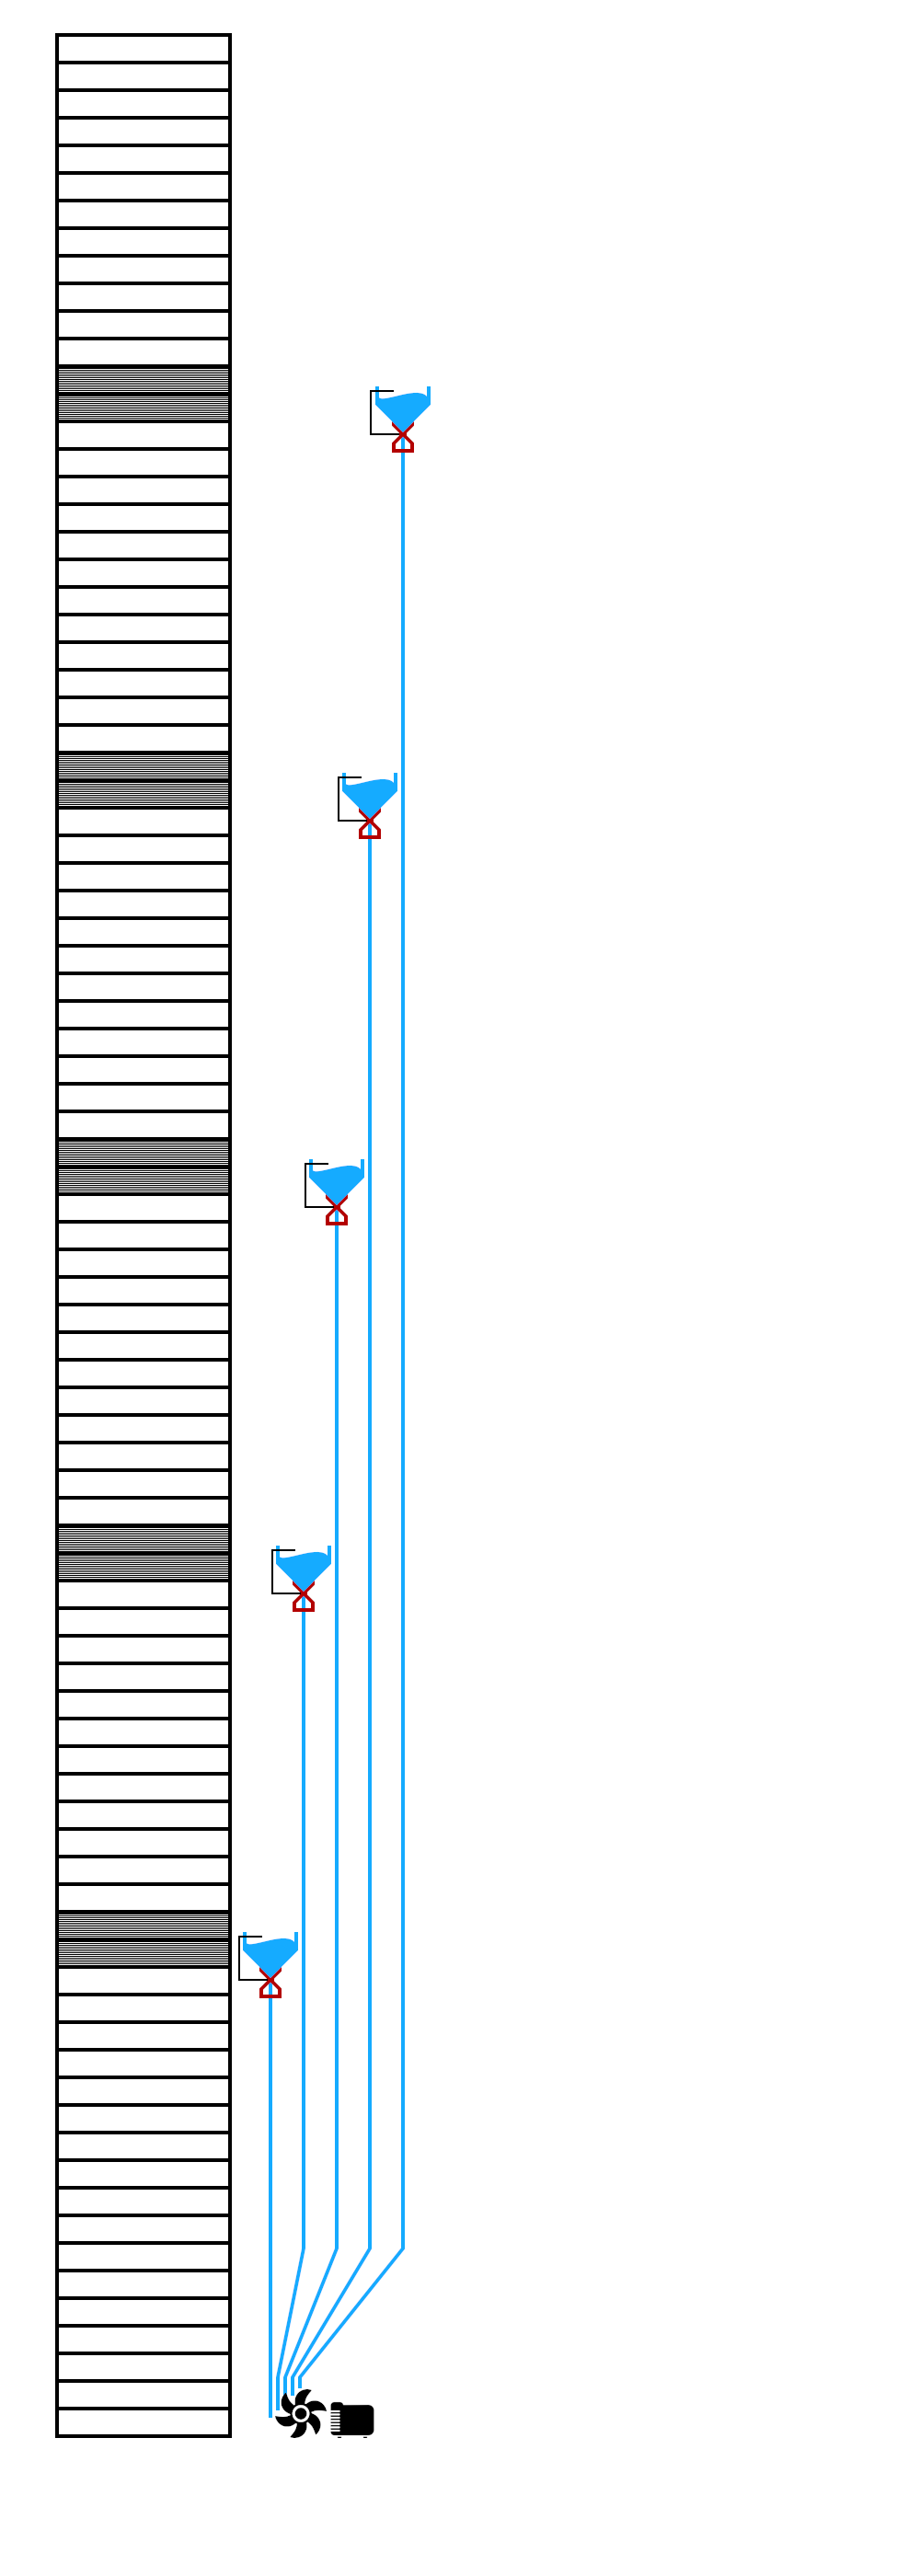
\includegraphics[width=0.48\textwidth]{grobkonzept2}
  \end{center}
  \caption{Schema Grobkonzept 2}
\end{wrapfigure}




Um zu verhindern, dass es in den Tanks zu Ablagerungen kommt, ist der Boden der Tanks trichterförmig. Ablagerungen werden dadurch beim Öffnen des Ventils weggespült. Sollte es trotzdem nötig sein, die Tanks zu reinigen, gibt es einen Bypass, mit dem das Abwasser am Tank vorbeigeführt werden kann.
Er kann dann entleert und gereinigt oder repariert werden. Auch die Turbine hat einen Bypass, der Wartungsarbeiten ermöglicht.

Jeder Tank ist mit einem Überlauf ausgestattet, der verhindert, dass ein Tank zu voll wird wenn z.B. der Ablauf verstopft ist. Das überschüssige Abwasser wird dann in einem Rohr in die Fallleitung wenige Stockwerke tiefer geleitet. Von dort gelangt es in den nächsten Abwassertank. Der Füllstandsensor im Tank erkennt, wenn der Pegel zu hoch wird und sendet eine Warnung.
Falls aus irgendeinem Grund mehr als eines der Ventile gleichzeitig geöffnet würde, könnte es zu einem Rückstau kommen, bei dem Abwasser durch die Druckleitungen vom höher gelegenen Tank in einen tieferen fliesst. Um dies zu verhindern, werden in den Druckleitungen Einwegventile eingebaut. Der höchstgelegene Tank benötigt kein solches Ventil. 

Ein Kontrollsystem steuert die Anlage und überwacht die Energiegewinnung und schreitet bei Störungen ein. Die Gewonnene Energie kann ins Netz zurück gespeist werden.

\bigskip

\textbf{Vorteile:} 									\newline
+	Luftwiderstand nur während Füllung				\newline
+	Nur eine Turbine									\newline
+	Keine AC-DC-AC Umwandlung						\newline
+	geregelte Wasserflussmenge						\newline

\textbf{Nachteile:}									\newline
-	braucht sehr viel Platz 							\newline
-	bauliche Massnahmen								\newline
-	Luftwiderstand während Füllung					\newline
- 	lange Druckleitungen								\newline
-	Abwasser der untersten 17 Stockwerke ungenutzt	\newline
\WFclear

\subsection{Grobkonzept 3} \label{subsec:grobkonzept3}

\begin{table}[H]
\begin{tabular}{>{\columncolor{hgelb}}l>{\columncolor{dgelb}}l>{\columncolor{hgelb}}llllll>{\columncolor{hgruen}}l>{\columncolor{dgruen}}l>{\columncolor{hgruen}}ll}
%GELBE KOLONNE						BLAUE UND PINKIGE KOLONNE										GRUENE KOLONNE
\titleCell{hgelb}{\textbf{Turbine}}	&&\titleCell{hblau}{\textbf{Elektrotechnik}}					&&\titleCell{hgruen}{\textbf{Abwassertechnik}}&\\
&\textbf{Turbinentyp}				&&&\cC{hblau}	&\cC{dblau}\textbf{Wechselrichter}	&\cC{hblau}	&&&\textbf{Tanks}				&&\\
&Pelton								&&&\cC{hblau}	&\cC{dblau}\textbf{Ventilsteuerung}	&\cC{hblau}	&&&Ablassentile					&&\\
&\textbf{Generatortyp}				&&&\cC{hblau}	&\cC{dblau}							&\cC{hblau}	&&&Entlüftung					&&\\
&Gleichstrom						&&&\titleCell{hblau}{ }											&&&Trichterförmig				&&\\
&\textbf{Anzahl}					&&&&&															&&&Füllstandssensor				&&\\
%ACHTUNG WEISSER ZWISCHENRAUM
&1									&&&\titleCell{hpink}{\textbf{Bedienung}}						&&&Notüberlauf					&&\\
&									&&&\cC{hpink}	&\cC{dpink}\textbf{Anzeige}			&\cC{hpink}	&&&\textbf{Druckleitungen}		&&\\
&									&&&\cC{hpink}	&\cC{dpink}der Füllstände			&\cC{hpink}	&&&Druckfestigkeit >40 bar		&&\\
&									&&&\cC{hpink}	&\cC{dpink}der Aktuellen Leistung	&\cC{hpink}	&&&\textbf{Bypass}				&&\\
&									&&&\cC{hpink}	&\cC{dpink}\textbf{Ventilsteuerung}	&\cC{hpink}	&&&für Tanks					&&\\
&									&&&\cC{hpink}	&\cC{dpink}							&\cC{hpink}	&&&für Turbine					&&\\
\titleCell{hgelb}{ }				&&\titleCell{hpink}{ }											&&\titleCell{hgruen}{ }&
\end{tabular}
\end{table}

Dieses Grobkonzept ist fast identisch zu Grobkonzept 2. Es gibt wieder einen oder mehrere Tanks, in denen das Abwasser zwischengespeichert wird. Allerdings gibt es nicht nur eine Turbine, sondern bei jedem Tank eine. Das Abwasser fliesst also immer von einem Tank in durch die Turbine in den darunterliegenden. Bei Grobkonzept 1 kann es relativ lange dauern, bis die Rohre komplett mit Wasser gefüllt sind. Bis das der Fall ist, kommt es zu Luftwiderstand in der Leitung. Bei jedem Tank eine Turbine einzubauen hat den Vorteil, dass die Rohre kürzer sind und so nach öffnen des Ventils schneller komplett mit Wasser gefüllt werden. So wird die Zeit verkürzt, in der Luftwiderstand auftritt. 

Vorteile 								\newline
+	Luftwiderstand tritt kürzer auf 	\newline
Nachteile	 							\newline
-	Braucht viel Platz					\newline
-	Grössere Bauliche Massnahmen nötig	\newline
-	Verstopfungsgefahr					\newline
-	Mehrere Turbinen nötig				


\subsection{Nutzwertanalyse} \label{subsec:nutzwertanlyse}
\renewcommand{\arraystretch}{1.5}
\newcommand{\vtcl}[1]{\rotatebox{90}{#1}}%\newcommand{\vtcl}[1]{\rotatebox{90}{\textbf{#1}}}
%\newcommand{\diagL}[1]{\diagbox{\hspace{#1}}{\hspace{#1}}}
Das Team hat blabla...
\begin{table}[H]
\small
\begin{tabular}{l|llllll|rr}
&\vtcl{1.1. Wirkungsgrad}&\vtcl{1.2. Leistung}&\vtcl{1.3. Komplexität}&\vtcl{2.1. Verstopfungsgefahr}&\vtcl{2.2. Platzbedarf}&\vtcl{2.3. Wartung}&\vtcl{Total}&\vtcl{Prozent}\\
\hline
1.1. Wirkungsgrad		&\cellcolor{black}	&0.5					&0.5					&0					&0.5					&0.5					&2.		&13\%\\
1.2. Leistung			&0.5					&\cellcolor{black}	&1					&1					&1					&1					&4.5		&30\%\\
1.3. Komplexität			&0.5					&0					&\cellcolor{black}	&0					&0					&0.5					&1.0		&6.5\%\\
2.1. Verstopfungsgefahr	&1					&0					&1					&\cellcolor{black}	&0					&1					&3		&20\%\\
2.2. Platzbedarf			&0.5					&0					&1					&1					&\cellcolor{black}	&1					&3.5		&24\%\\
2.3. Wartung				&0.5					&0					&0.5					&0					&0					&\cellcolor{black}	&1.0		&6.5\%\\
\hline
\multicolumn{7}{c}{}&\textbf{15}&\textbf{100}\%\\
\end{tabular}
\end{table}
\begin{scriptsize}
Zeile-Kriterium ist wichtiger als Spalten-Kriterium 1\\
Zeile-Kriterium ist gleich wichtig wie Spalten-Kriteriium 0.5\\
Zeile-Kriterum ist weniger wichtig wie Spalternkriterium 0\\
\end{scriptsize}
\newcolumntype{C}[1]{>{\centering}p{#1}}
\begin{table}[H]
\small
\begin{tabular}{lC{1.2cm}C{1.2cm}C{1.2cm}C{1.2cm}C{1.2cm}l}
\multicolumn{7}{c}{\textbf{Erfüllungsgrad}}\\
\hline
&min.&&mittel&&max.&\\
&\textbf{1}&\textbf{2}&\textbf{3}&\textbf{4}&\textbf{5}&Messgrösse\\
\hline
1.1. Wirkungsgrad				&<50&51-60&61-70&71-80&>81&\%\\
1.2. Leistung					&<40&40-44&45-50&51-54&>55&kWh\\
1.3. Schlichtheit				&>16&15-12&11-8&7-4&<3&Anz. versch. Teile\\
2.1. Verstopfungssicherheit		&gering&mässig&mittel&erhöht&hoch&a)\\
2.2. Platzsparung				&gering&mässig&mittel&erhöht&gross&Schätzung m\textsuperscript{3}\\
2.3. Wartung						&52-13&12-6&5-2&1&0&b)\\
\end{tabular}
\end{table}
\begin{scriptsize}
a) Abschätzung via Recherche\\
b) geschätze Frequenz [1\textbackslash J]
\end{scriptsize}

\newpage
\renewcommand\arraystretch{1.5}
\newcolumntype{R}[1]{>{\HY\RaggedLeft}p{#1}}
\newcolumntype{L}[1]{>{\HY\RaggedRight}p{#1}}
\renewcommand{\vtcl}[1]{\rotatebox{90}{\textbf{#1}}}
\begin{table}[H]
\small
\rotatebox{90}{
%|R{1.2cm}R{0.4cm}R{0.8cm} \scriptsize
%|R{1cm}R{0.2cm}R{0.5cm} \tiny
\begin{tabular}{L{3.5cm}R{1.5cm}L{0.8cm}|R{1.4cm}R{0.5cm}r|R{1.4cm}R{0.5cm}r|R{1.4cm}R{0.5cm}r|R{1.4cm}R{0.5cm}r|}%|R{1cm}R{0.5cm}R{0.8cm}
&&Max&\multicolumn{3}{c}{Grobkonzept 1}&\multicolumn{3}{c}{Grobkonzept 2}&\multicolumn{3}{c}{Grobkonzept 3}&\multicolumn{3}{c}{Grobkonzept 4}\\
\textbf{Zielkriterium}&\vtcl{Gewichtung}&\vtcl{Nutzwert}&\vtcl{Wert}&\vtcl{Erfüllungsgrad}&\vtcl{Nutzwert}&\vtcl{Wert}&\vtcl{Erfüllungsgrad}&\vtcl{Nutzwert}&\vtcl{Wert}&\vtcl{Erfüllungsgrad}&\vtcl{Nutzwert}&\vtcl{Wert}&\vtcl{Erfüllungsgrad}&\vtcl{Nutzwert}\\
\hline
&&&&&&&&&&&&&&\\
\rowcolor{hellgrau}
\multicolumn{3}{l|}{\textbf{Elektrotechnik}}&\multicolumn{3}{r|}{}&\multicolumn{3}{r|}{}&\multicolumn{3}{r|}{}&\multicolumn{3}{r|}{}\\
%										%G1 Wert		%G1 Erf.		G1 Nutz			%G2 Wert		%G2 Erf.		G2 Nutz			%G3 Wert		%G3 Erf.		G2 Nutz			%G4 Wert		%G4 Erf.		G4 Nutz
Wirkungsgrad			&13\%		&0.650	&32\%		&1			&0.13			&67.2\%		&3			&0.39			&64.1\%		&3			&0.39			&80\%		&4			&0.52\\
Leistung				&30\%		&1.500	&21.5kWh		&1			&0.3	0			&44.6kWh		&2			&0.6	0			&42.6kWh		&2			&0.60			&53.1kWh		&4			&1.20\\
Schlichtheit			&6.5\%		&0.325	&6			&4			&0.26			&15			&2			&0.26			&14			&2			&0.20			&6			&4			&0.26\\
%&&&&&&&&&&&&&&\\
\rowcolor{hellgrau}
\multicolumn{3}{l|}{\textbf{Abwassertechnik}}&\multicolumn{3}{r|}{}&\multicolumn{3}{r|}{}&\multicolumn{3}{r|}{}&\multicolumn{3}{r|}{}\\
Verstopfungssicherheit&20\%		&1.000	&mässig		&2			&0.40			&mässig		&2			&0.4	0			&mässig		&2			&0.40			&mittel		&3			&0.60\\
Platzsparung			&24\%		&1.200	&erhöht		&4			&0.96			&mässig		&2			&0.48			&gering		&1			&0.24			&erhöht		&5			&1.20\\
Wartung				&6.5\%		&0.325	&5			&2			&0.26			&3			&2			&0.26			&1			&4			&0.20			&1			&4			&0.20\\
&&&&&&&&&&&&&&\\
\hline
Summe				&100.0\%		&5.000	&			&			&2.31			&			&			&2.39			&			&			&2.03			&			&			&3.98\\
Erfüllungsgrad [\%]	&&100.0				&			&			&46				&			&			&48				&			&			&40				&			&			&79\\
\multicolumn{3}{l}{\textbf{Rangfolge}}&\multicolumn{3}{r|}{\textbf{4}}&\multicolumn{3}{r|}{\textbf{2}}&\multicolumn{3}{r|}{\textbf{3}}&\multicolumn{3}{r|}{\textbf{1}}\\
\end{tabular}
}
\end{table}





